\section{Memcached}

The purpose of this chapter is to benchmark and evaluate memcached performance. Firstly, we will examine performance under default configuration of both the server and the client. Secondly, threading will be explored in relation to latency and throughput. Thirdly, the effect of memcached's \texttt{group size} will be explored in relation to performance. Additionally, configuration of receive and transmit queues will be explored and finally, an execution model of multiple processes will be visited in order to establish a comparison baseline. Throughout the benchmarks, we will be focusing cache performance which meets desired the QoS.


\subsection{Default Performance}

Firstly, it is essential to establish a performance baseline of \emph{memcached} under high utilization. In order to establish the baseline, a default configuration of memcached will be used with the exception of the amount of memory allocated for exclusive use by the application. The \emph{memcached} application will be started with
\begin{lstlisting}
memcached -d -p 11120 -m 6144
\end{lstlisting} specifying the port and the amount of memory to be used by the application.

To find a saturation point, we can increase the number of connections linearly and analyze the results. To load test the cache, we execute the following command on all client servers simultaneously.
\begin{lstlisting}
  memtier -s nsl200 -p 11120 -c <connections> -t 2
    --random-data
    --key-minimum=100
    --key-maximum=10000
\end{lstlisting}

The effect will be to generate random data with keys between the specified ranges and send requests to the server in two simultaneous threads.


\subsubsection{Default Throughput vs Latency}

Firstly, we are interested in the relationship between throughput and latency shown in Figure \ref{fig:memcached-default-latency-vs-ops}. The mean latency and the 99th percentile latency are plotted against corresponding number of operations (throughput). We can observe that as the number of operations increases so does latency. Additionally, latency (both 99th percentile and mean) increase linearly until a saturation point is reached when a further increase in throughput is met with an exponentially larger increase in latency. The highest throughput achieved under quality of service restriction of 99th percentile latency under 1 millisecond is 375,000 operations per second. The highest level of throughput corresponds to 84 simultaneous connections, or 12 connections per each client which is similar to benchmarks used in the literature \cite{lim2013thin}.

\begin{figure}[h]
    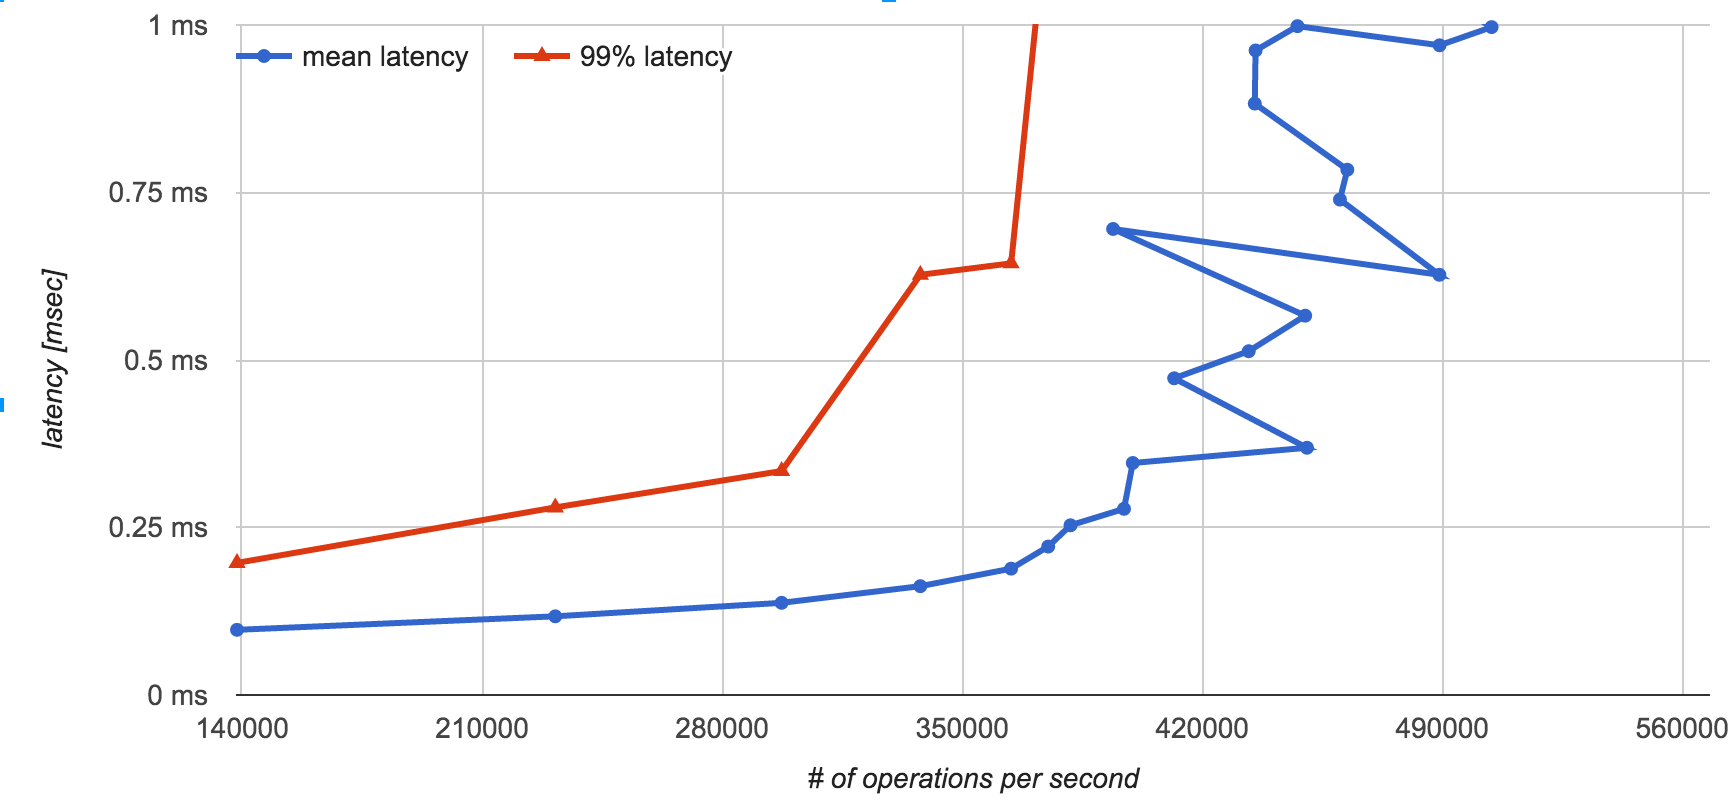
\includegraphics[width=\textwidth]{./res/5_default_latency_vs_ops.png}
    \caption{Mean latency and 99th percentile latency against throughput}
    \label{fig:memcached-default-latency-vs-ops}
\end{figure}


\subsubsection{Effect of Connections}
To understand the effect of a large number of connections on the cache performance, Figure \ref{fig:memcached-default_connections} shows the effect an increase in the total number of connections has on throughput, mean latency and the 99th percentile latency. The figure deliberately shows the behavior outside of the requires QoS requirements in order to better illustrate the impact on the cache under high load.

\begin{figure}[h]
    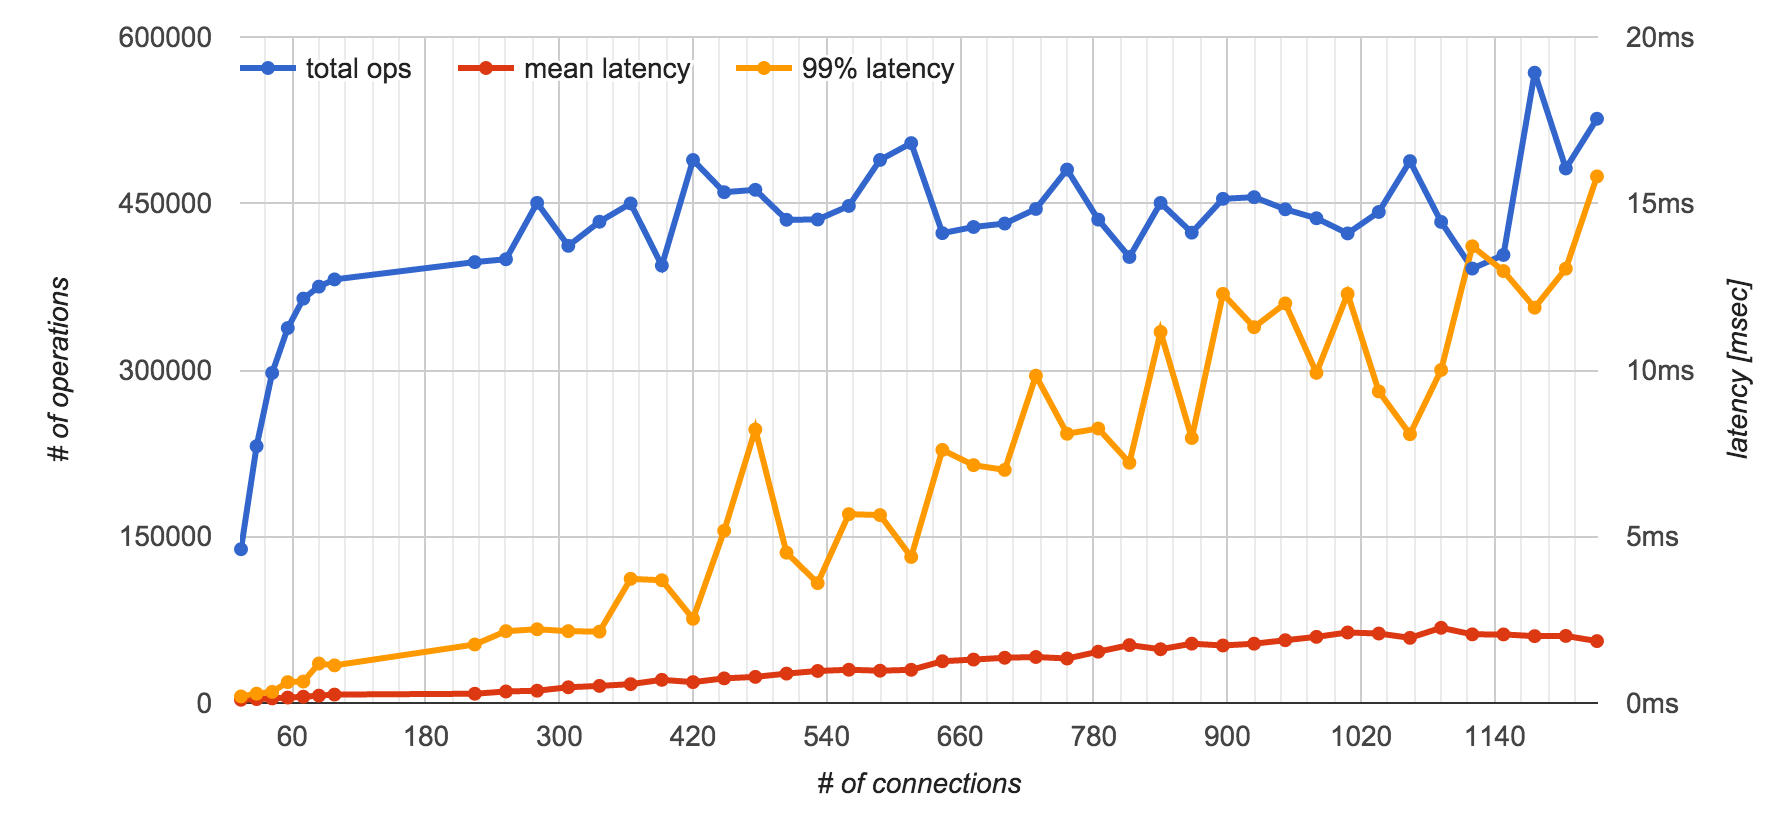
\includegraphics[width=\textwidth]{./res/5_default_connections.png}
    \caption{Throughput, Mean latency and 99th percentile against the number of connections}
    \label{fig:memcached-default_connections}
\end{figure}

Firstly, Figure \ref{fig:memcached-default_connections} displays the general trend an increased load has on throughput. As load increases, so does throughput. However, as the number of connections surpasses 100, the rate of increase in throughput for each increase the number of connections decreases. This is the saturation point of the cache, an increase in load yield disproportionate increase in throughput. Beyond the saturation point, the cache throughput fluctuates around 450,000 operations per second.

Secondly, the mean latency increases linearly with the number of connections (load). This is an expected behavior as the server experiences network stack queuing as well as increased resource requirements to process requests.

Thirdly, the 99th percentile latency increases linearly, with some fluctuations, against the increased server load. As the load gets higher, the fluctuation increases as well as the upper bound. This is due to some requests being queued for a long time before being processed, pushing the 99th percentile high.

We can observe that the server is capable of scaling much better until around 100 connections are reached. When the saturation point is surpassed, overall performance and quality of service degrades.


\subsubsection{Server CPU}
In order to be better understand the impact of memcached on the system, specifically the CPU usage, we consider a breakdown of CPU time spent in various areas of the operating system in Figure \ref{fig:memcached-default-cpu}.

\begin{figure}[h]
    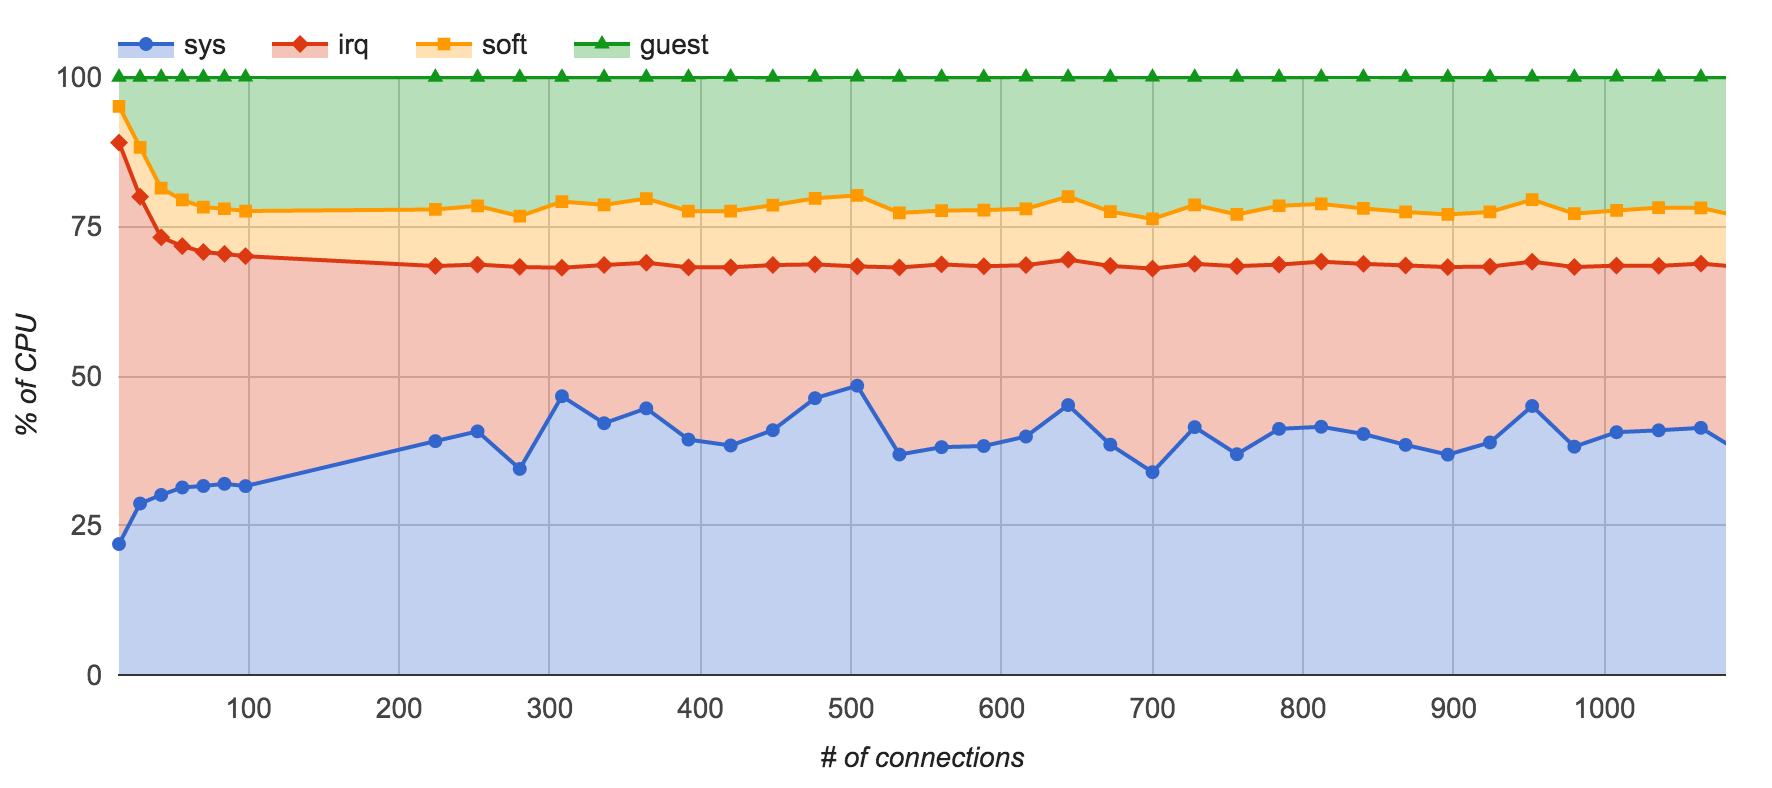
\includegraphics[width=\textwidth]{./res/5_default_cpu.png}
    \caption{CPU Time against number of connections}
    \label{fig:memcached-default-cpu}
\end{figure}

Firstly, we can observe that the effective footprint of memcached (\texttt{guest}) is relatively small compared to the rest. The CPU usage of memcached increases up until 100 connections at which point it remains fairly stable.

Secondly, the operating system (\texttt{sys}) increases as we increase the load. Fluctuations occur past 250 connections but the CPU usage by the system remains around 40 percent as the load is increased further. An increased number of connections requires additional resources to process incoming requests as well as process outgoing requests. The context switching from receiving and transmitting contributes to the high load from the system.

Thirdly, interrupt processing by the system (\texttt{irq}) decreases as we increase load, this is due to having more CPU available and therefore being able to process a higher number of interrupts per unit of time. As resources are required by the system and the memcached application, this number of interrupts processed per unit of time decreases as reflected by the proportion of CPU.

Finally, software interrupt footprint (\texttt{soft}) remains relatively stable throughout. The software interrupts correspond to running threads of the memcached application (4 threads by default) and are used for context switching.

From the breakdown in Figure \ref{fig:memcached-default-cpu}, we can conclude that memcached is not CPU heavy on its own. The large CPU footprint of running memcached under high load is tightly linked to performance of the network stack and the underlying hardware processing network requests rather than the application itself. This observation is consistent with findings in MICA \cite{lim2014mica}.


\subsection{Memcached Thread Scalability}
Memcached, as a high performance object cache, is designed to be executed on a parallel architecture. It implements scalability through the use multiple threads allowing memcached to utilize many core architectures. Therefore, the next step in scaling a memcached deployment is to provision a larger number of threads for the application.

Memcached execution model is capable of processing incoming and outgoing requests in parallel, however, operations executed require a global application lock to be acquired. Therefore, the expected number of threads maximising throughput while minimizing latency can be expected to be achieved when memcached is provisioned with the same number of threads as hardware CPU cores which is also suggested by Leverich and Kozyrakis \cite{leverich2014reconciling}.

Utilizing findings from the previous section, a configuration with 84 connections can be used to generate a consistent load while the number of threads provisioned for memcached can be varied. Therefore, we can set up each benchmark client as follows:

\begin{lstlisting}
  memtier -s nsl200 -p 11120 -c 6 -t 2 -P memcache_binary
    --random-data
    --key-minimum=100
    --key-maximum=10000
\end{lstlisting}

The server in turn is configured as follows:
\begin{lstlisting}
  memcached -d -p 11120 -m 6144 -t <thread_count>
\end{lstlisting}

Where the number of threads is progressively increased.

\subsubsection{Throughput \& Latency}

Figure \ref{fig:memcached-threads} shows the relationship between throughput, mean latency and 99th percentile latency in relation to the number of threads used by a memcached application.

\begin{figure}[h]
    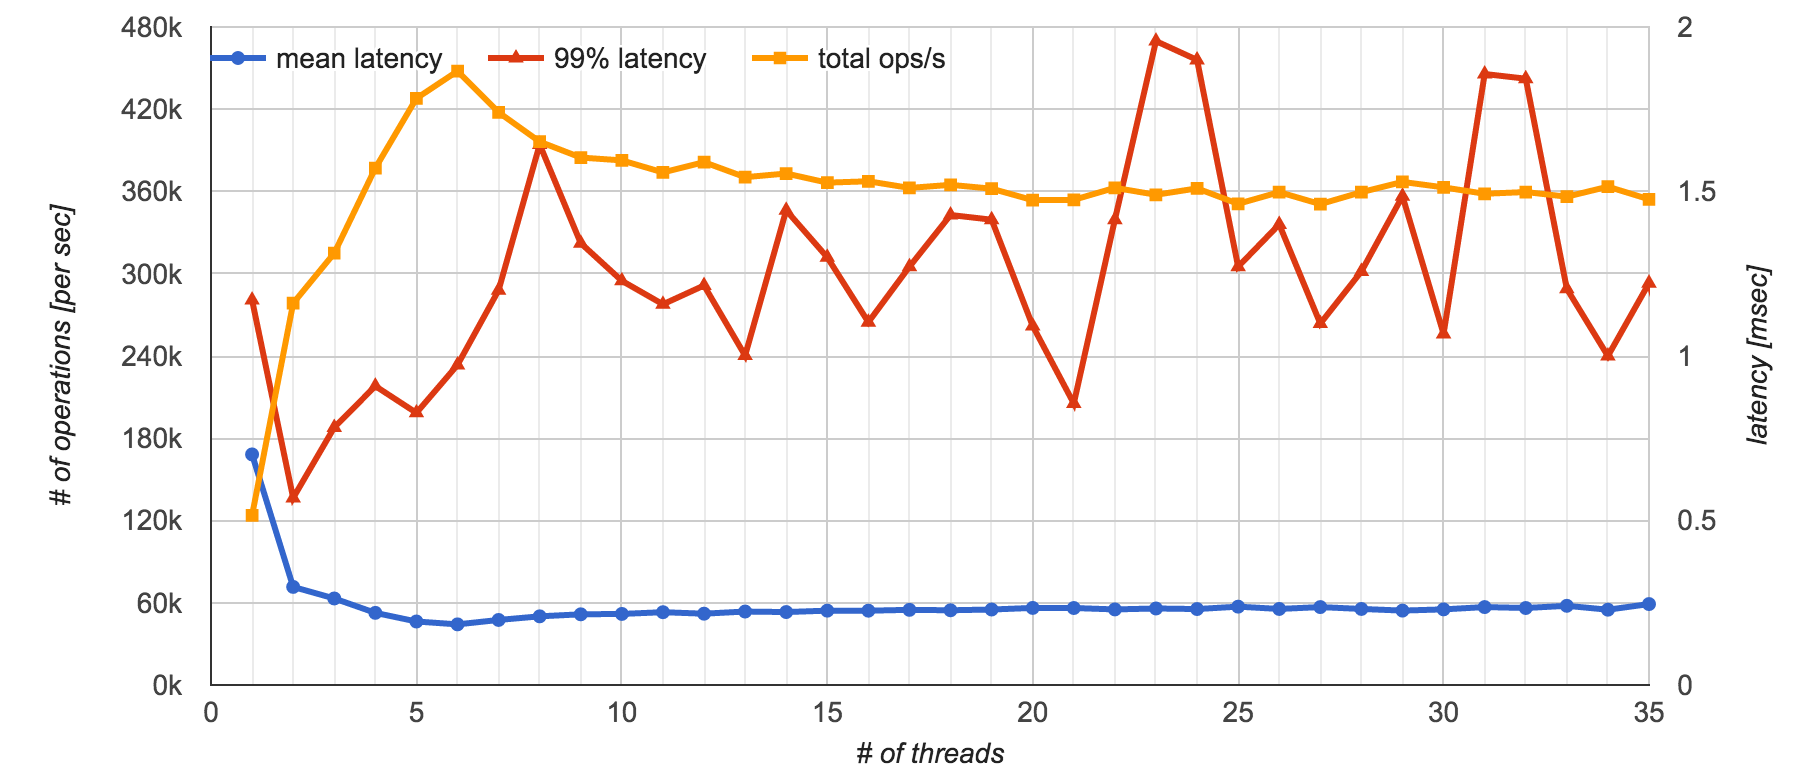
\includegraphics[width=\textwidth]{./res/5_memcached_threads.png}
    \caption{Memcached Thread Scaling}
    \label{fig:memcached-threads}
\end{figure}

Firstly, we can observe that throughput increases as thread count increases until we reach 6 threads where it peaks at 450k requests per second. As we increase thread count further, throughput decreases. This behavior corresponds with our expectation that performance is maximized when there are as many threads as CPU cores.

Secondly, mean latency decreases as the number of threads is increased reaching a minimum of 0.1843 milliseconds at 6 threads. With more threads, the mean latency increases steadily.

Thirdly, the 99th percentile latency decreases as we increase the number of threads from 1 to 2, reaching a minimum and increasing as the number of threads increases. At 6 threads, we reach a 99th percentile latency of 0.973 which satisfies the QoS requirements under 1 millisecond.

Indeed, as expected we have been able to obtain the highest throughput and achieve the quality of service requirements with 6 threads, as many as CPU cores on the host. Beyond 6 threads, the overhead of context switching between threads increases processing time and reduces throughput.

\subsubsection{CPU Time}

\begin{figure}[h]
    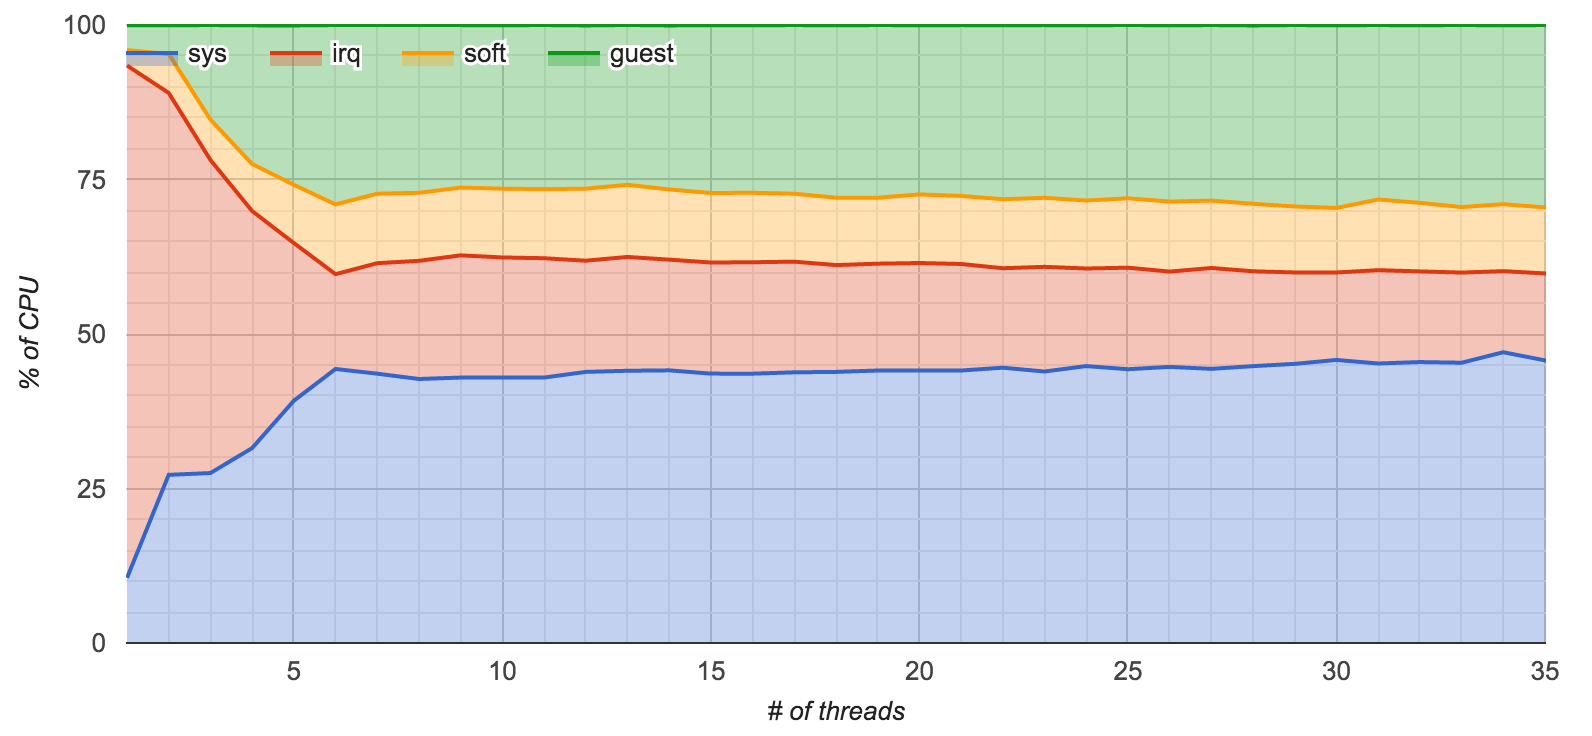
\includegraphics[width=\textwidth]{./res/5_threads_cpu.png}
    \caption{Memcached CPU Time against Number of Threads}
    \label{fig:memcached-threads-cpu}
\end{figure}

Analyzing the CPU usage in Figure \ref{fig:memcached-threads-cpu} as we increase the number of threads, we can observe that initially a large portion of the CPU time is spent servicing hardware interrupts (\textit{irq}). Therefore, the OS is handling incoming traffic interrupts from the NIC. As the number of threads increases, an increasingly larger portion of CPU time is spent processing system calls and context switching (\textit{sys}). This is reasonable as a larger number of threads will require context switching and concurrency management provided by the operating system. We can see that time spent processing hardware interrupts (\textit{irq}) decreases which has the effect of increasing latency as packets remained queued up in the NIC for longer before the OS manages to schedule the interrupt to be serviced. Furthermore, we can observe that software interrupts (\textit{soft}) CPU time progressively increases until we reach 6 threads and remains stable as the number of threads grows further. The initial increase is reasonable as we are demanding more threads to processed simultaneously, past this point the percentage remains stable as we have reached a saturation point in terms of scalability and server performance. Finally, memcached (\textit{guest}) follows a similar pattern as software interrupts. Usage increases until 6 threads are used and saturates further. This is further indicative of the inability to efficiently scale the number of threads past the point at which memcached uses the same number of threads as CPU cores.

\subsubsection{Thread evaluation}
Comparing results obtain from thread scalability with the results from the default configuration of memcached, we have been able to increase throughput from 375k to 450k requests per second while maintaining the desired QoS under 1ms.



\subsection{Thread pinning}
Thread pinning is the process of assigning a \textit{set\_irq\_affinity} to each individual thread. As suggested by Leverich and Kozyrakis, "pinning memcached threads to distinct cores greatly improves load balance, consequently improving tail latency." \cite{leverich2014reconciling} and therefore the reasonable next step in optimizing memcached performance is to attempt thread pinning and analyse the results obtained.

By default, when a new process is started, its affinity is set to all available CPUs. We can discover a given process affinity by executing the following command where \textit{pid} is the process identifier.

\begin{lstlisting}
    taskset -p <pid>
\end{lstlisting}


"A Memcache instance started with n threads will spawn n + 1 threads of which the first n are worker threads and the last is a maintenance thread used for hash table expansion under high load factor." \cite{solarflarememcached}. We can discover memcached threads used for request processing using the following command where \textit{tid} is the thread id discovered previously \cite{solarflarememcached}.
\begin{lstlisting}
    ps -p <memcache-pid> -o tid= -L | sort -n | tail -n +2 | head -n -1
\end{lstlisting}

Given the best performance under QoS constraints of 1ms found in the previous section is memcached with 6 threads, the following benchmark will be using this best configuration in order the analyze the impact of thread pinning.

\subsubsection{Throughput vs Latency}

\begin{figure}[h]
    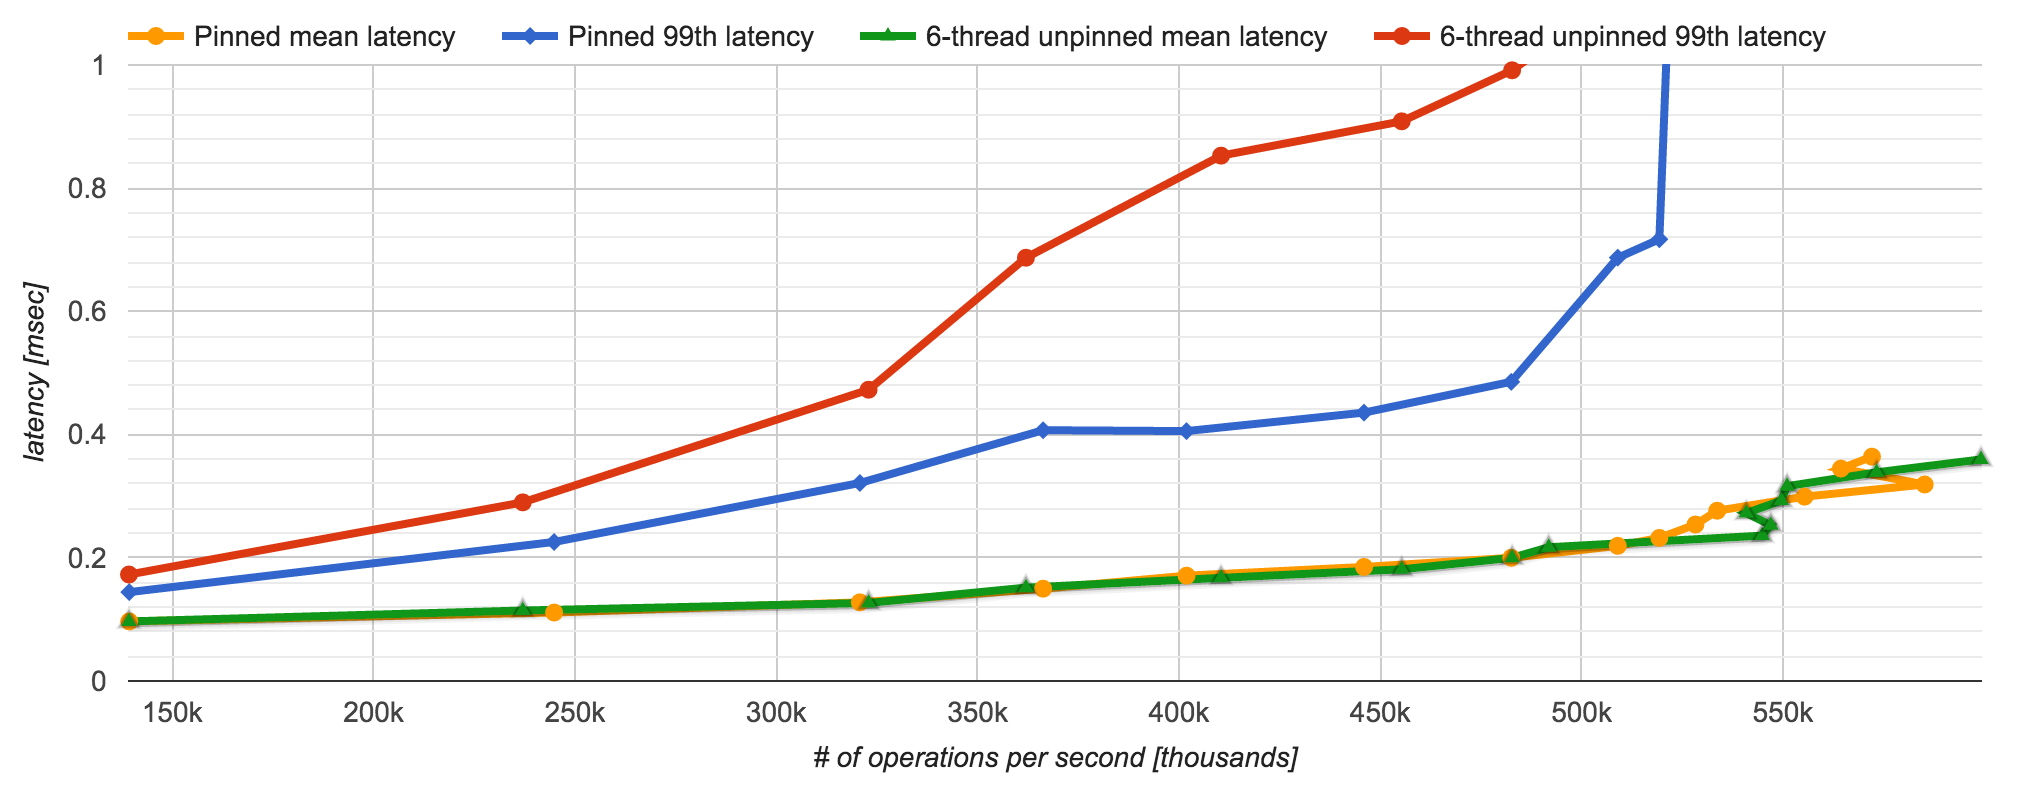
\includegraphics[width=\textwidth]{./res/5_threads_pinned.png}
    \caption{Memcached Pinned Threads vs Unpinned}
    \label{fig:memcached-threads-pinned}
\end{figure}

Figure \ref{fig:memcached-threads-pinned} shows the impact thread pinning has on mean and 99th percentile latency against throughput.

Firstly, the mean latency of both pinned and unpinned benchmarks remains very similar as throughput increases.

Secondly, the 99th percentile latency is lower in the case of pinned threads than unpinned. The pattern holds as throughput increases up until the required QoS boundary.

Furthermore, the throughput has also increased reaching 520k requests per second compared to 475k requests per second in the case of unpinned threads. This pattern is further confirmed by  Leverich and Kozyrakis \cite{leverich2014reconciling}.

The reason for a significant improvement in the tail latency is reduced contention for access to receive and transmission queues in the network stack. Given memcached's design of running \textit{t} threads for request processing and \textit{1} thread for hash table expansion under high load, the result may be two or more request processing threads scheduled on the same CPU core while the hash table expansion thread is scheduled to run alone on a core. Pinning threads prevents this scenario from occurring as well as creates a direct mapping between each receive and transmission queue in the network stack to the memcached thread, reducing need for context switching.


\subsection{Group Size}
Memcached provides a configuration option \textit{-R} to set the group size used inside memcached. The group size defines the ``Maximum number of requests per event, limits the number of requests process for a given connection to prevent starvation (default: 20)'' \cite{interactive2006memcached}. This in effect means the number of requests that will be processed from a single connection before memcached switches to a different connection to achieve a fair policy.

In order to benchmark the effects of an increased group size, we

\begin{figure}[h]
    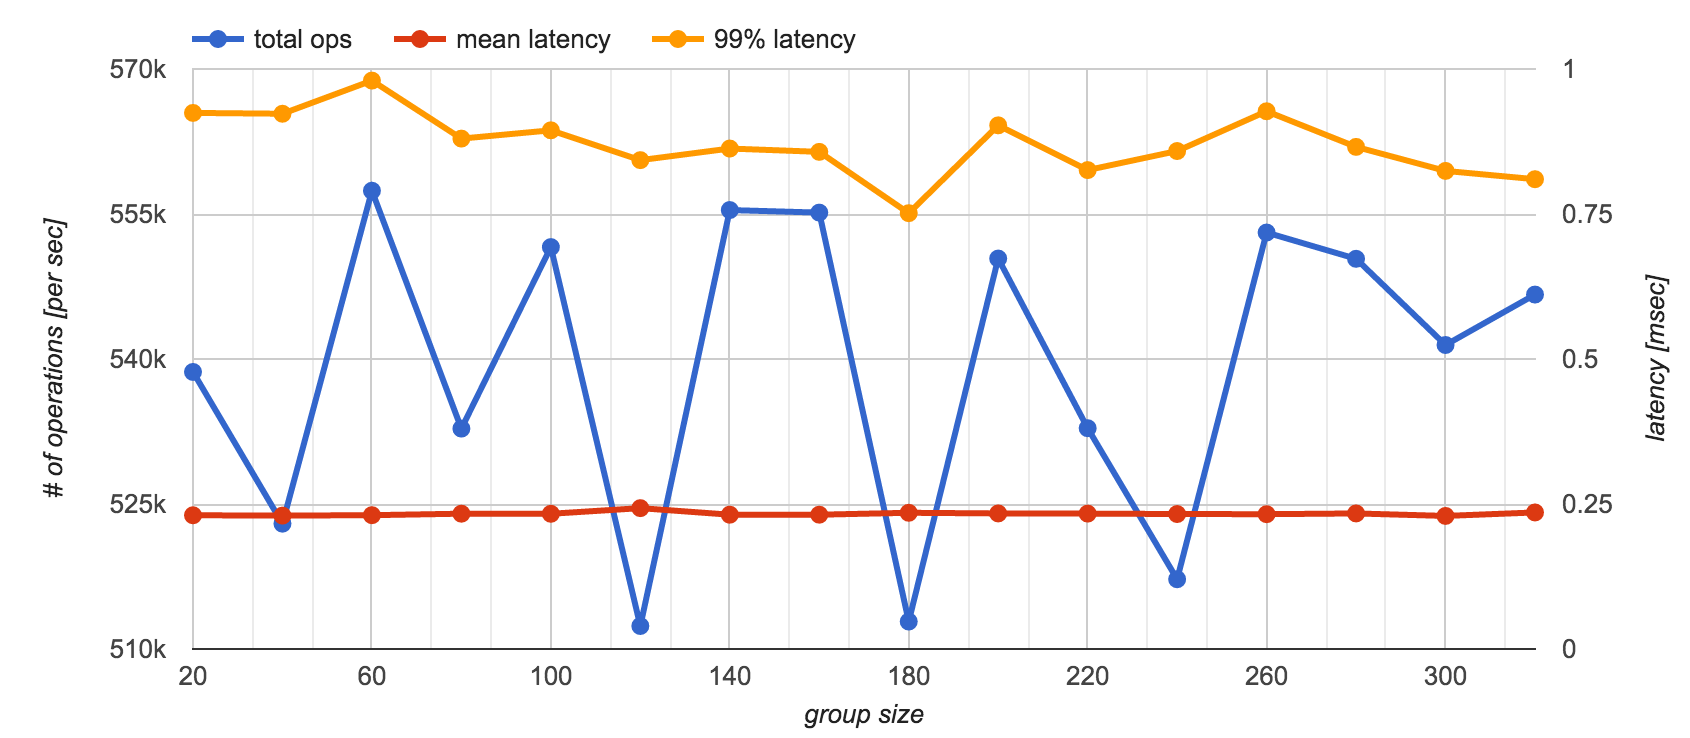
\includegraphics[width=\textwidth]{./res/5_memcached_group_size.png}
    \caption{Memcached Latency, 99th percentile latency and throughput against group size}
    \label{fig:memcached_group_size}
\end{figure}

Figure \ref{fig:memcached_group_size} shows the relationship between throughput, mean latency and 99th percentile latency.
